
\begin{abstract}
  Authoring Semantic Web documents such as ontologies or SPARQL queries is error-prone, often leading to interoperability issues, validation failures, or incorrect reasoning.
  To address these challenges, we present the Semantic Web Language Server (SWLS), a tool for Semantic Web practitioners that integrates IDE-like functionalities such as real-time syntax validation, intelligent autocompletion, and SHACL-based diagnostics into modern code editors.
  SWLS follows the Language Server Protocol, allowing seamless integration with popular code editors such as Visual Studio Code and NeoVim, while currently supporting multiple Semantic Web formats including Turtle, JSON-LD and SPARQL.
  This demo accompanies an accepted ESWC 2025 resource paper and showcases SWLS in an interactive web-based environment, where users can explore its features across four dedicated editor panels: (i) an RDF instance data editor, (ii) an ontology editor, (iii) a SHACL shape editor and (iv) a SPARQL query editor. 
  The demo highlights SWLS’s ability to detect syntax and semantic errors, suggest completions based on dereferenced ontologies, and assist users in writing coherent SPARQL queries.
  By improving the development workflow and addressing common pitfalls, SWLS aims to enhance the usability of Semantic Web technologies and facilitate broader adoption.
\keywords{Language Server, IDE, Tool, Linked Open Vocabularies, Semantic Web}
\end{abstract}

\textbf{URL:} \url{https://ajuvercr.github.io/semantic-web-lsp/} 

\textbf{Licenses:} MIT License


\section{Introduction}%
\label{sec:introduction}

The Semantic Web comprises a variety of syntax formats for expressing and querying data, such as Turtle, JSON-LD, and SPARQL. 
These formats enable representing semi-structured data in an interoperable way.
However, authoring and editing documents following these formats is prone to human error, which can lead to non-interoperability, validation failures or incorrect reasoning outcomes.
For instance, mistyping the URI of a prefix can alter the entire meaning of an RDF document, rendering it non-interoperable with other datasets. 

Some open services such as Linked Open Vocabularies (LOV)~\cite{LOV2017} or \href{https://prefix.cc}{prefix.cc} provide both human-oriented and programmatic interfaces to look up exact definitions of predicates and classes, offering a reliable reference for avoiding such errors.
Tools such as YASGUI~\cite{yasgui,10.1007/978-3-642-41242-4_7} and \href{https://query.wikidata.org/}{query.wikidata.org} provide robust web-based functionalities for editing SPARQL queries.
However these do not integrate into local development environments nor support multiple formats.

In this demo paper, we showcase the Semantic Web Language Server (SWLS), a language server based on the Language Server Protocol (LSP), designed to assist editors in handling Semantic Web documents. 
SWLS runs locally, allowing for quick development cycles and seamless integration into developer workflows, including popular code editors such as Visual Studio Code and NeoVim. 
Moreover, SWLS supports multiple Semantic Web formats such as Turtle, SPARQL and JSON-LD.
It is also designed with extensibility in mind, making it a versatile solution. 
This demo paper accompanies an accepted ESWC 2025 resource paper, where more details about the SWLS architecture design can be found.

All code is licensed under the MIT License and available on GitHub\footnote{\url{https://github.com/ajuvercr/semantic-web-lsp}}.

\section{Semantic Web Language Server}

SWLS follows the Language Server Protocol (LSP)~\cite{IntroToLsp}\footnote{\url{https://microsoft.github.io/language-server-protocol/}},
a protocol allowing one server implementation to interact with different editors, reducing complexity from $O(M*N)$ to $O(M+N)$,
with $M$ editors and $N$ languages.

The server communicates using JSON-RPC, enabling bidirectional messaging between the editor and server for handling features such as autocompletion, highlighting, and diagnostics.
Most modern editors support LSP, including Visual Studio Code and NeoVim.
The server is implemented in Rust, and allows to be compiled to WASM (portable low level byte code) that integrates into browsers.

SWLS is designed for flexibility, allowing support for multiple file formats with maximal code reuse. 
It uses an entity component system (ECS) to build a layered architecture~\cite{10.1145/3550355.3552452}, following a traditional \textit{Feature Execution Flow}.

\begin{enumerate}
  \item The \textit{Parse} step handles parsing the document (emitting potential syntax errors) and deriving defined triples and prefixes.

  \item The \textit{Traverse} step derives information from the triples, such as defined properties, classes and SHACL shapes. 
    Starting from the defined prefixes, this step also finds the used ontologies using the public LOV api, these ontologies are added to the ECS, functioning as sources for defined properties and classes.
        This step also emits dignostics, notifying the editor of potential mistakes in the document, including undefined prefixes, and shape violations (using the Rudof~\cite{labra2022rudof} library).

  \item The \textit{Process} step extracts all required information from the previous steps and translates it into a response for the current request.
        Currently SWLS handles autocompletion (predicates, classes and prefixes), renaming and hover.
\end{enumerate}
The ECS design enables reusing the systems for the \textit{Traverse} and \textit{Process} steps across different languages, 
requiring only the \textit{Parse} step to be implemented for each file format.

\section{Demo}
\renewcommand{\textfloatsep}{5pt}  % Space between figure and text
\begin{figure}[tb]
    \centering
    \begin{subfigure}{0.48\textwidth}
      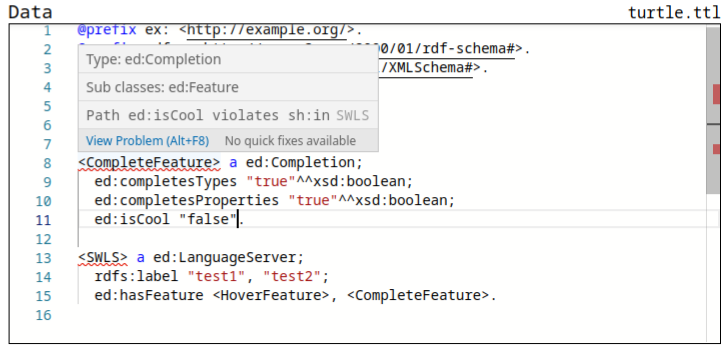
\includegraphics[width=\textwidth]{./images/hover.png}
      \caption{SWLS shows the user type information on hover as well as diagnostics}
      \label{hover}
    \end{subfigure}
    \hfill
    \begin{subfigure}{0.48\textwidth}
      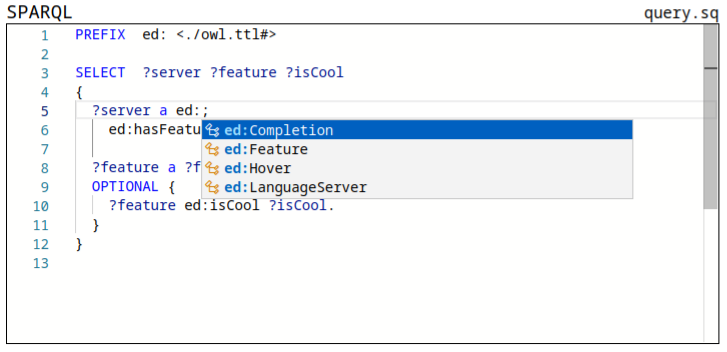
\includegraphics[width=\textwidth]{./images/class.png}
      \caption{SWLS completes a class when the user wants to write a class}
      \label{class_completion}
    \end{subfigure}
    \hfill
    \begin{subfigure}{0.48\textwidth}
      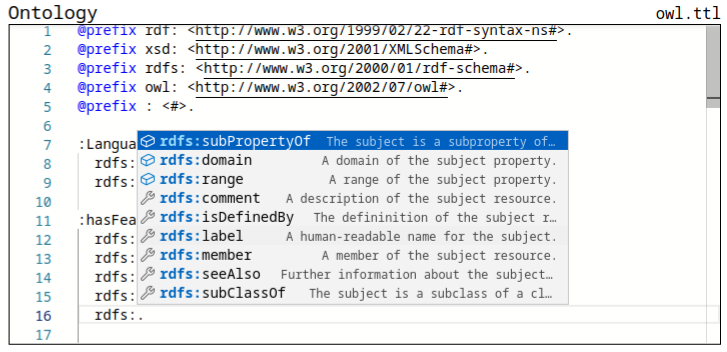
\includegraphics[width=\textwidth]{./images/property.png}
      \caption{SWLS completes properties, first the properties with the correct domain}
      \label{property_completion}
    \end{subfigure}
    \hfill
    \begin{subfigure}{0.48\textwidth}
      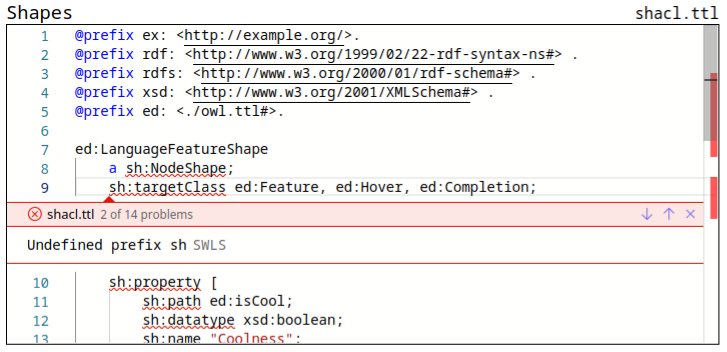
\includegraphics[width=\textwidth]{./images/undefined.png}
      \caption{SWLS notifies the user of undefined prefixes}
      \label{undefined_prefix}
    \end{subfigure}
    \caption{
      Demo application that shows the usage of SWLS. Features include hover information, autocompletion and diagnostics.
    }\label{lst:Demo}
\end{figure}

The demo consists of an online application at \url{https://ajuvercr.github.io/semantic-web-lsp/}.
The app has four editor panels, each with a different purpose, and runs entirely in browser. The editors use the opensource Monaco editor\footnote{\url{https://github.com/microsoft/monaco-editor}}
that communicate with the language server compiled to WASM.
% : a data pane for authoring RDF data, an ontology pane for vocabulary management, a shape pane for SHACL constraints, and a query pane for SPARQL queries.
%
% All panes are treated equally, except for the query pane, which is designed for SPARQL rather than Turtle, but uses the same SWLS instance.

\begin{enumerate}
  \item The \textbf{data panel} represents an RDF dataset, where users can author and edit linked data.
    Errors detected via SHACL validation are highlighted, as shown in Figure \ref{hover}.
    Users can correct these errors either by adding missing triples or modifying the shape definitions in the shape panel.
  \item The \textbf{ontology panel} contains a playground ontology that describes language servers.
    It is linked to the data panel using a prefix import, enabling autocompletion of relevant properties, as shown in Figure \ref{property_completion}.
  \item The \textbf{query panel} allows users to write SPARQL queries against the data. 
    While SWLS does not execute queries, it provides autocompletion for classes and properties, as depicted in Figure \ref{class_completion}.
  \item The \textbf{shape panel} includes SHACL constraints imported into the data panel via the \texttt{owl:imports} property. 
    As shown in Figure \ref{undefined_prefix}, SWLS alerts users to undefined prefixes, and typing a prefix triggers autocompletion suggestions, adding the import statement.
\end{enumerate}

Users can also try the language server on local editors.
For VSCode, users can install the Semantic Web LSP\footnote{\url{https://marketplace.visualstudio.com/items?itemName=ajuvercr.semantic-web-lsp}}.
Setting up the server with NeoVim requires installing the language server with cargo (Rust's package manager) and configuring the language server with \textit{lspconfig}.

\section{Conclusion}

The Semantic Web Language Server (SWLS) introduces IDE-like functionalities for authoring Semantic Web documents, supporting multiple formats and providing a local development workflow. 
By integrating features such as real-time validation, context-aware autocompletion, and SHACL-based diagnostics, SWLS lowers the chance of errors in local documents.
Unlike existing tools, SWLS runs locally and extends beyond Turtle, offering a more flexible and powerful authoring experience.
This work not only addresses current limitations in Semantic Web tooling but also paves the way for broader adoption of semantic technologies by reducing barriers and improving usability.


